\documentclass[a4paper,12pt]{article}\usepackage[]{graphicx}\usepackage[]{color}
%% maxwidth is the original width if it is less than linewidth
%% otherwise use linewidth (to make sure the graphics do not exceed the margin)
\makeatletter
\def\maxwidth{ %
  \ifdim\Gin@nat@width>\linewidth
    \linewidth
  \else
    \Gin@nat@width
  \fi
}
\makeatother

\definecolor{fgcolor}{rgb}{0.345, 0.345, 0.345}
\newcommand{\hlnum}[1]{\textcolor[rgb]{0.686,0.059,0.569}{#1}}%
\newcommand{\hlstr}[1]{\textcolor[rgb]{0.192,0.494,0.8}{#1}}%
\newcommand{\hlcom}[1]{\textcolor[rgb]{0.678,0.584,0.686}{\textit{#1}}}%
\newcommand{\hlopt}[1]{\textcolor[rgb]{0,0,0}{#1}}%
\newcommand{\hlstd}[1]{\textcolor[rgb]{0.345,0.345,0.345}{#1}}%
\newcommand{\hlkwa}[1]{\textcolor[rgb]{0.161,0.373,0.58}{\textbf{#1}}}%
\newcommand{\hlkwb}[1]{\textcolor[rgb]{0.69,0.353,0.396}{#1}}%
\newcommand{\hlkwc}[1]{\textcolor[rgb]{0.333,0.667,0.333}{#1}}%
\newcommand{\hlkwd}[1]{\textcolor[rgb]{0.737,0.353,0.396}{\textbf{#1}}}%
\let\hlipl\hlkwb

\usepackage{framed}
\makeatletter
\newenvironment{kframe}{%
 \def\at@end@of@kframe{}%
 \ifinner\ifhmode%
  \def\at@end@of@kframe{\end{minipage}}%
  \begin{minipage}{\columnwidth}%
 \fi\fi%
 \def\FrameCommand##1{\hskip\@totalleftmargin \hskip-\fboxsep
 \colorbox{shadecolor}{##1}\hskip-\fboxsep
     % There is no \\@totalrightmargin, so:
     \hskip-\linewidth \hskip-\@totalleftmargin \hskip\columnwidth}%
 \MakeFramed {\advance\hsize-\width
   \@totalleftmargin\z@ \linewidth\hsize
   \@setminipage}}%
 {\par\unskip\endMakeFramed%
 \at@end@of@kframe}
\makeatother

\definecolor{shadecolor}{rgb}{.97, .97, .97}
\definecolor{messagecolor}{rgb}{0, 0, 0}
\definecolor{warningcolor}{rgb}{1, 0, 1}
\definecolor{errorcolor}{rgb}{1, 0, 0}
\newenvironment{knitrout}{}{} % an empty environment to be redefined in TeX

\usepackage{alltt}
\usepackage{mathtools,amsfonts,amssymb,cmbright,bm,commath,multicol}
\IfFileExists{upquote.sty}{\usepackage{upquote}}{}
\begin{document}

\normalsize 14D001 || Multiple Testing || Nandan Rao || 1/11/2016

\section{Distribution of p-value under the null}

\subsection{}


\section{Multiple testing under independence assumptions}

\subsection{}

Using the formula for distribution complements $\mathbb{P}(A^c) = 1 - \mathbb{P}(A)$, along with the definition for a given random variable y drawn from a uniform distribution spanning 0 to 1, and $\alpha \in [0, 1]$:

\begin{align*}
\mathbb{P}(y \leq \alpha) &= \alpha \\
\mathbb{P}(y > \alpha) &= 1 - \alpha
\end{align*}

The joint probability of a series of independent events is given by the product of their individual probabilities. If $\mathbb{P}(A_m)$ for all values of m are equal, this is equivalent to:

$$
\mathbb{P}(\cap_{i=1}^m) = \mathbb{P}(A)^m
$$

From which follows that for any series of independent draws from a uniform distribution, $y_1, ... y_m$:

\begin{align*}
\mathbb{P}(\cap_{i=1}^m \set{y_i > \alpha}) &= \mathbb{P}(y_1 > \alpha)^m \\
\mathbb{P}(\cap_{i=1}^m \set{y_i > \alpha}) &= (1 - \alpha)^m
\end{align*}

\subsection{}

We reject a single null hypothesis at significance level $\alpha$ with probability $\alpha$. The complement of rejecting a single null hypothesis is to accept a single null hypothesis, which we therefore do with probability $1 - \alpha$. To accept ALL null hypotheses, from a set of m of hypothesis tests with I.I.D. uniformly distributed p-values, is therefore given by:

$$
\mathbb{P}(\textrm{accepting all null hypothises}) = (1 - \alpha)^m
$$

The complement of accepting evey null hypothesis, would be to reject one or more null hypothesis:

\begin{align*}
\mathbb{P}(\textrm{reject one or more null hypotheses}) &= 1 - \mathbb{P}(\textrm{accepting all null nypothises}) \\
\mathbb{P}(\textrm{reject one or more null hypotheses}) &= 1 - (1 - \alpha)^m
\end{align*}


\subsection{}

Let $\alpha_0$ represent the significance level with which we reject each individual null hypothesis and $\alpha$ represent the probability that we reject one or more null hypotheses from a set of hypotheses with I.I.D. uniform p-values. Starting from our equation above, we can find $\alpha_0$ in terms of $\alpha$:

\begin{align*}
\alpha &= 1 - (1 - \alpha_0)^m \\
1 - \alpha &= (a - \alpha_0)^m \\
(a - \alpha)^{\frac{1}{m}} &= 1 - alpha_0 \\
\alpha_0 &= 1 - (1 - \alpha)^{\frac{1}{m}}
\end{align*}

\subsection{}

\begin{knitrout}
\definecolor{shadecolor}{rgb}{0.969, 0.969, 0.969}\color{fgcolor}
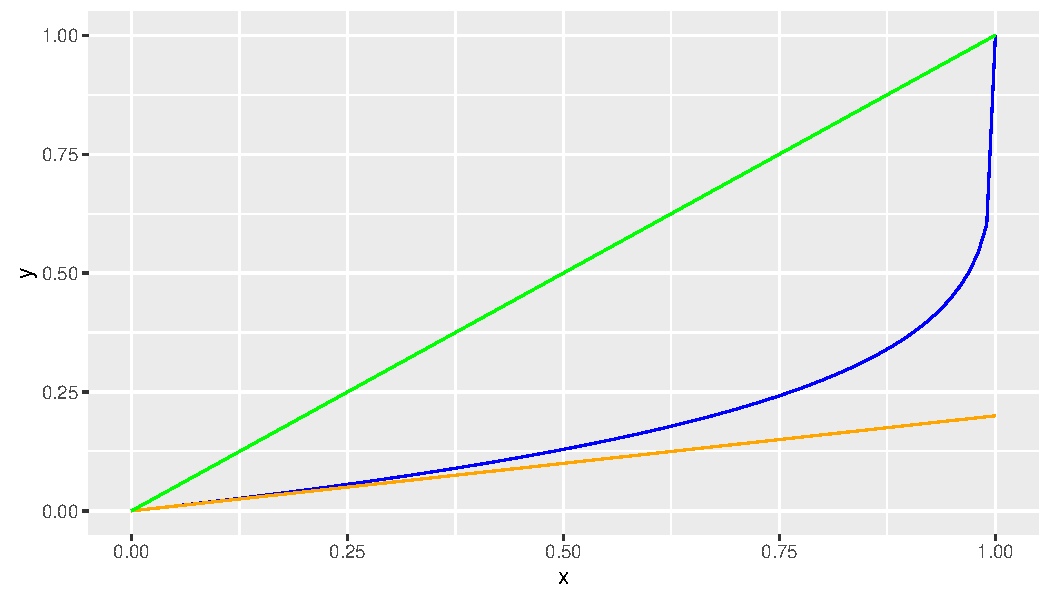
\includegraphics[width=\maxwidth]{figure/coefficients-1} 

\end{knitrout}

\subsection{}

We consider all situations where $\alpha \in [0,1]$ and all $m \geq 1$ to prove that $f_2(\alpha) \leq f_1(\alpha)$:


\subsection{}
Under independence assumptions, as shown in (2.3), the significance level needed for each test, $\alpha_0$, is shown to be $1 - (1 - \alpha)^{\frac{1}{m}}$. Making now correction for multiple testing, we follow the generic per-comparisson error rate (PCER), and accept or reject each individual test at $\alpha_0 = \alpha$. As shown in (2.5):

$$
\alpha &\geq 1 - (1 - \alpha)^{\frac{1}{m}}
$$

And from that we can see that the significance level needed for each individual test if we consider each test p-value as being I.I.D. from a uniform distribution, is much lower if we consider the joint probability of all our tests and aim to keep the probability of rejecting one or more null hypothesis at our significance level, then if we make no correction for the joint probability of our multiple tests.

\section{Proof of Bonferroni Correction}

Using Boole's Inequality, we can rewrite the probability of rejecting one or more null hypotheses to be:

$$
\mathbb{P}_{C - H} \big( \cup_{i=1}^m \set{ p_i(\bm{Y}_i) \leq \alpha } \big) \leq \sum_{i=1}^m \mathbb{P}(\bm{Y}_i \leq \alpha)
$$

If we consider $\bm{Y}_1, ... \bm{Y}_m$ to be p-values drawn from a uniform distribution from 0 to 1, we can state that the probability of any given $\bm{Y}_i \leq \alpha$, where $\alpha \in [0,1]$, is equal to $\alpha$. This leads to the following:

\begin{align*}
\mathbb{P}_{C - H} \big( \cup_{i=1}^m \set{ p_i(\bm{Y}_i) \leq \alpha } \big) &\leq \sum_{i=1}^m \mathbb{P}(\bm{Y}_i \leq \alpha) \\
\mathbb{P}_{C - H} \big( \cup_{i=1}^m \set{ p_i(\bm{Y}_i) \leq \alpha } \big) &\leq \sum_{i=1}^m \alpha \\
\mathbb{P}_{C - H} \big( \cup_{i=1}^m \set{ p_i(\bm{Y}_i) \leq \alpha } \big) &\leq m\alpha \\
\end{align*}

\section{Ordered p-values}



\end{document}
